%Input preamble
%Style
\documentclass[12pt]{article}
\usepackage[top=1in, bottom=1in, left=1in, right=1in]{geometry}
\parindent 22pt
\usepackage{fancyhdr}

%Packages
\usepackage{adjustbox}
\usepackage{amsmath}
\usepackage{amsfonts}
\usepackage{amssymb}
\usepackage[english]{babel}
\usepackage{bm}
\usepackage[table]{xcolor}
\usepackage{tabu}
\usepackage{color,soul}
\usepackage[utf8x]{inputenc}
\usepackage{makecell}
\usepackage{longtable}
\usepackage{multirow}
\usepackage[normalem]{ulem}
\usepackage{etoolbox}
\usepackage{graphicx}
\usepackage{tabularx}
\usepackage{ragged2e}
\usepackage{booktabs}
\usepackage{caption}
\usepackage{fixltx2e}
\usepackage[para, flushleft]{threeparttablex}
\usepackage[capposition=top]{floatrow}
\usepackage{subcaption}
\usepackage{pdfpages}
\usepackage{pdflscape}
\usepackage[sort&compress]{natbib}
\usepackage{bibunits}
\usepackage[colorlinks=true,linkcolor=darkgray,citecolor=darkgray,urlcolor=darkgray,anchorcolor=darkgray]{hyperref}
\usepackage{marvosym}
\usepackage{makeidx}
\usepackage{setspace}
\usepackage{enumerate}
\usepackage{rotating}
\usepackage{epstopdf}
\usepackage[titletoc]{appendix}
\usepackage{framed}
\usepackage{comment}
\usepackage{xr}
\usepackage{titlesec}
\usepackage{footnote}
\usepackage{longtable}
\newlength{\tablewidth}
\setlength{\tablewidth}{9.3in}
\usepackage[bottom]{footmisc}
\usepackage{stackengine}
\newcommand\barbelow[1]{\stackunder[1.2pt]{$#1$}{\rule{1ex}{.085ex}}}
\usepackage{titletoc}
\usepackage{accents}
\usepackage{arydshln }
\usepackage{titletoc}
\titlespacing{\section}{.2pt}{1ex}{1ex}
\setcounter{section}{0}
\renewcommand{\thesection}{\arabic{section}}


\makeatletter
\pretocmd\start@align
{%
  \let\everycr\CT@everycr
  \CT@start
}{}{}
\apptocmd{\endalign}{\CT@end}{}{}
\makeatother
%Watermark
\usepackage[printwatermark]{xwatermark}
\usepackage{lipsum}
\definecolor{lightgray}{RGB}{220,220,220}
\definecolor{dimgray}{RGB}{105,105,105}

%\newwatermark[allpages,color=lightgray,angle=45,scale=3,xpos=0,ypos=0]{Preliminary Draft}

%Further subsection level
\usepackage{titlesec}
\titleformat{\paragraph}
{\normalfont\normalsize\bfseries}{\theparagraph}{1em}{}
\titlespacing*{\paragraph}
{0pt}{3.25ex plus 1ex minus .2ex}{1.5ex plus .2ex}

\titleformat{\subparagraph}
{\normalfont\normalsize\bfseries}{\thesubparagraph}{1em}{}
\titlespacing*{\subparagraph}
{0pt}{3.25ex plus 1ex minus .2ex}{1.5ex plus .2ex}

%Functions
\DeclareMathOperator{\cov}{Cov}
\DeclareMathOperator{\sign}{sgn}
\DeclareMathOperator{\var}{Var}
\DeclareMathOperator{\plim}{plim}
\DeclareMathOperator*{\argmin}{arg\,min}
\DeclareMathOperator*{\argmax}{arg\,max}

%Math Environments
\usepackage{amsthm}
\newtheoremstyle{mytheoremstyle} % name
    {\topsep}                    % Space above
    {\topsep}                    % Space below
    {\color{black}}                   % Body font
    {}                           % Indent amount
    {\itshape \color{dimgray}}                   % Theorem head font
    {.}                          % Punctuation after theorem head
    {.5em}                       % Space after theorem head
    {}  % Theorem head spec (can be left empty, meaning ?normal?)

\theoremstyle{mytheoremstyle}
\newtheorem{assumption}{Assumption}
\renewcommand\theassumption{\arabic{assumption}}

\theoremstyle{mytheoremstyle}
\newtheorem{assumptiona}{Assumption}
\renewcommand\theassumptiona{\arabic{assumptiona}a}

\newtheorem{assumptionb}{Assumption}
\renewcommand\theassumptionb{\arabic{assumptionb}b}

\newtheorem{assumptionc}{Assumption}
\renewcommand\theassumptionc{\arabic{assumptionc}c}

\theoremstyle{mytheoremstyle}
\newtheorem{lemma}{Lemma}

\theoremstyle{mytheoremstyle}
\newtheorem{proposition}{Proposition}

\theoremstyle{mytheoremstyle}
\newtheorem{corollary}{Corollary}

%Commands
\newcommand\independent{\protect\mathpalette{\protect\independenT}{\perp}}
\def\independenT#1#2{\mathrel{\rlap{$#1#2$}\mkern2mu{#1#2}}}
\newcommand{\overbar}[1]{\mkern 1.5mu\overline{\mkern-1.5mu#1\mkern-1.5mu}\mkern 1.5mu}
\newcommand{\equald}{\ensuremath{\overset{d}{=}}}
\captionsetup[table]{skip=10pt}
%\makeindex

%Table, Figure, and Section Styles
\captionsetup[figure]{labelfont={bf},name={Figure},labelsep=period}
\renewcommand{\thefigure}{\arabic{figure}}
\captionsetup[table]{labelfont={bf},name={Table},labelsep=period}
\renewcommand{\thetable}{\arabic{table}}
\titleformat{\section}{\centering \normalsize \bf}{\thesection.}{0em}{}%\titlespacing*{\subsection}{0pt}{0\baselineskip}{0\baselineskip}
\renewcommand{\thesection}{\arabic{section}}

\titleformat{\subsection}{\flushleft \normalsize \bf}{\thesubsection}{0em}{}
\renewcommand{\thesubsection}{\arabic{section}.\arabic{subsection}}

%No indent
\setlength\parindent{24pt}
\setlength{\parskip}{5pt}

%Logo
%\AddToShipoutPictureBG{%
%  \AtPageUpperLeft{\raisebox{-\height}{\includegraphics[width=1.5cm]{uchicago.png}}}
%}

\newcolumntype{L}[1]{>{\raggedright\let\newline\\\arraybackslash\hspace{0pt}}m{#1}}
\newcolumntype{C}[1]{>{\centering\let\newline\\\arraybackslash\hspace{0pt}}m{#1}}
\newcolumntype{R}[1]{>{\raggedleft\let\newline\\\arraybackslash\hspace{0pt}}m{#1}} 

\newcommand{\mr}{\multirow}
\newcommand{\mc}{\multicolumn}

%\newcommand{\comment}[1]{}

\begin{document}


\title{\Large \textbf{Does Entrepreneurship Mitigate or Exacerbate Social Mobility? }}
\author{Yi Ling}

\date{\today}

\maketitle

\thispagestyle{empty} 
\doublespacing
\thispagestyle{empty} 

\section{Research Question}
This proposal aims to compare the outcomes of two types of entrepreneurs:  nascent entrepreneurs and entrepreneurs whose family is also self-employed, and examine whether the first type faces lower intergenerational mobility than the second type, in other words, can people from a non-entrepreneur family background climb up the social ladder through choosing to start a business?

\section{Data Description}
There are many data sources that provide information on income, profits, and investments for entrepreneurs and their family backgrounds. One prominent dataset is the Panel Study of Income Dynamics (PSID), a longitudinal household survey that began in 1968 and covers a nationally representative sample of over 18,000 individuals from 5,000 families in the United States. \citet{quadrini1999importance,fairlie1999absence} both use the  (PSID) to study the financial and human capital transition across generations. 

The second dataset is the Current Population Survey (CPS), which is an important source of labor force data in the United States. To study the entrepreneurship trend, \citet{jiang2023skill, sanchez2023decline, bento2023barriers} both used CPS and found the decline trend in the entrepreneur population. Before calculating the income, investment of two types of entrepreneurs, I also calculated the population trend to ensure my definition of entrepreneurs is the same as previous literature. First, I only included the people who have an active employment status. Second, I define entrepreneurs as "self-employed" from the data. For family background, I only consider parents' employment status first, then I merge parents' employment information with the original data. Figure \ref{nascent} shows the population trend of nascent entrepreneurs, which is consistent with the results from \citet{jiang2023skill, sanchez2023decline}.

\begin{figure}[htp!]
    \centering
    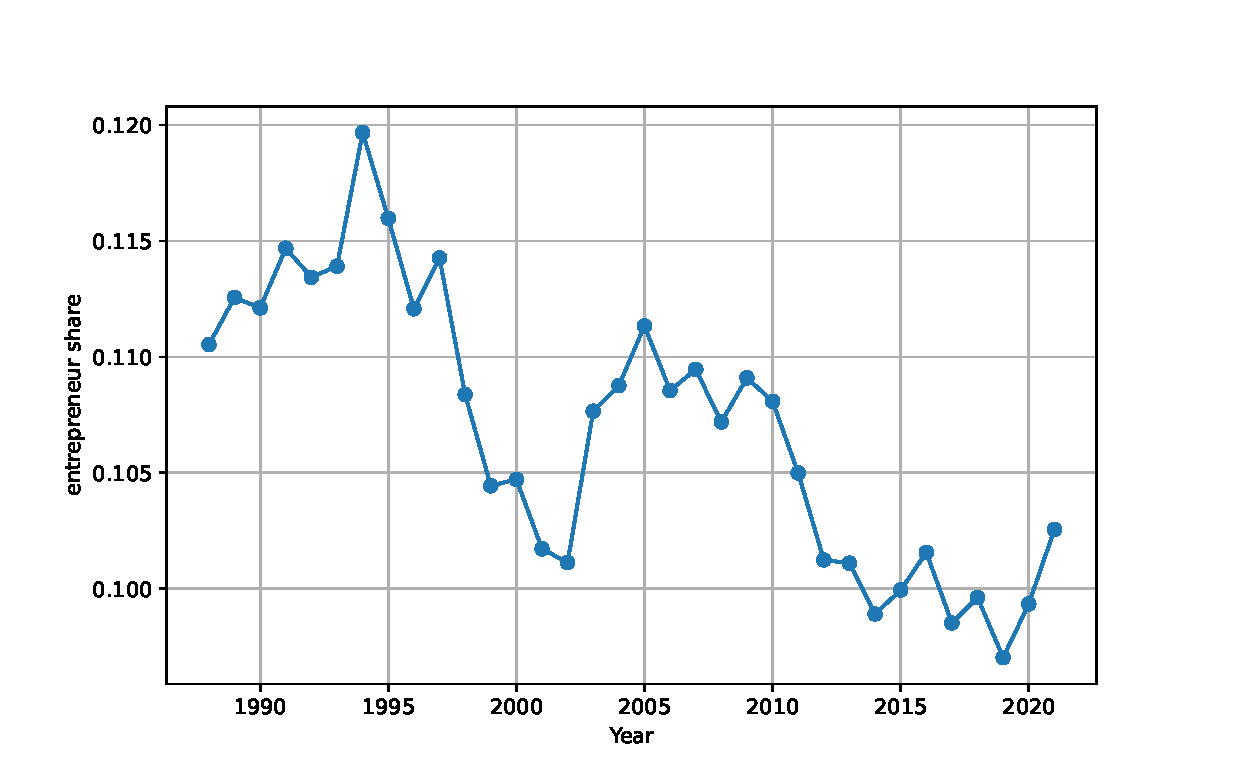
\includegraphics[width=0.5\textwidth]{nascententrepreneursharecps.eps}
    \caption{Population Trend of Nascent Entrepreneurs}
    \label{nascent}
\end{figure}


Another dataset is also helpful to identify the entrepreneur trend over time but cannot provide detailed information about the entrepreneurs' families. For instance, Survey of Consumer Finance (SCF) is also widely used to observe the entreprenuers population and investment \citep{moskowitz2002returns, cagetti2006entrepreneurship}, however, the question in the inverview is " How did you (or your family living here) first acquire this business; was it bought or invested in, started by you,  inherited, given to you, or some other way?", therefore, we cannot identify whether the business is started by that person or his family.


\bibliographystyle{apalike} 
\bibliography{references}

\end{document}

